
%********************************************************************
% Appendix
%*******************************************************
% If problems with the headers: get headings in appendix etc. right
%\markboth{\spacedlowsmallcaps{Appendix}}{\spacedlowsmallcaps{Appendix}}
\chapter{Appendix A Manual Data Entry Tool GUI}
\label{app:mantoolgui}

The GUI used by the manual data entry tool.

As shown by \autoref{fig:mtLogin} the user is first required to log on. Note that for ease of use all details, except passwords, are stored on the client machine, using cookies.
 \begin{figure}[H]
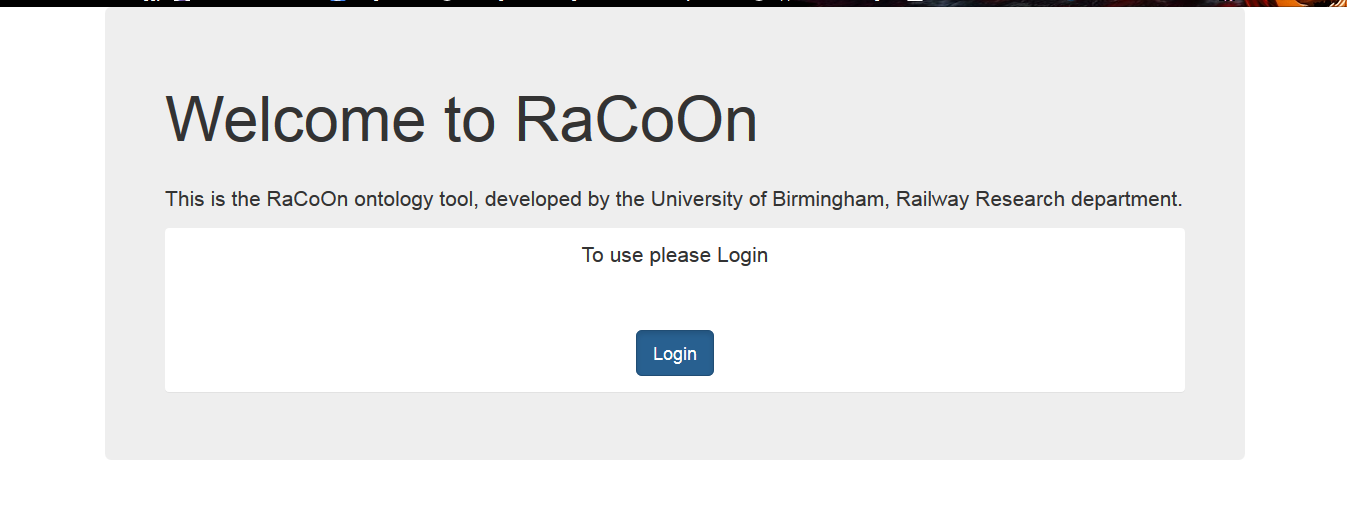
\includegraphics[max height=\textheight,max width=\linewidth]{gfx/manToolWelcome}
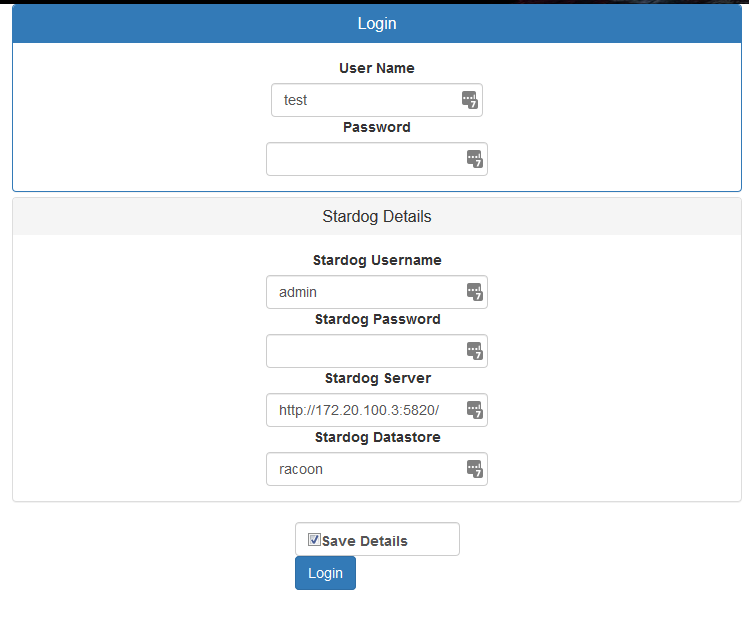
\includegraphics[max height=0.5\textheight,max width=\linewidth]{gfx/manToolLogin}
\caption{Manual Data Entry tool welcome and login screens}
\label{fig:mtLogin}
\end{figure}

If log-in is successful the user is presented with the main menu, as shown in \autoref{fig:mtMainMenu}. 
 \begin{figure}[!h]
\myfloatalign
{
\includegraphics[max height=0.5\textheight,max width=\linewidth]{gfx/manToolInUse}} 
\caption[Manual Data Entry Tool]{Manual Data Entry Tool main menu}
\label{fig:mtMainMenu}
\end{figure}

\section{Add an item}

 \begin{figure}[!h]
\myfloatalign
{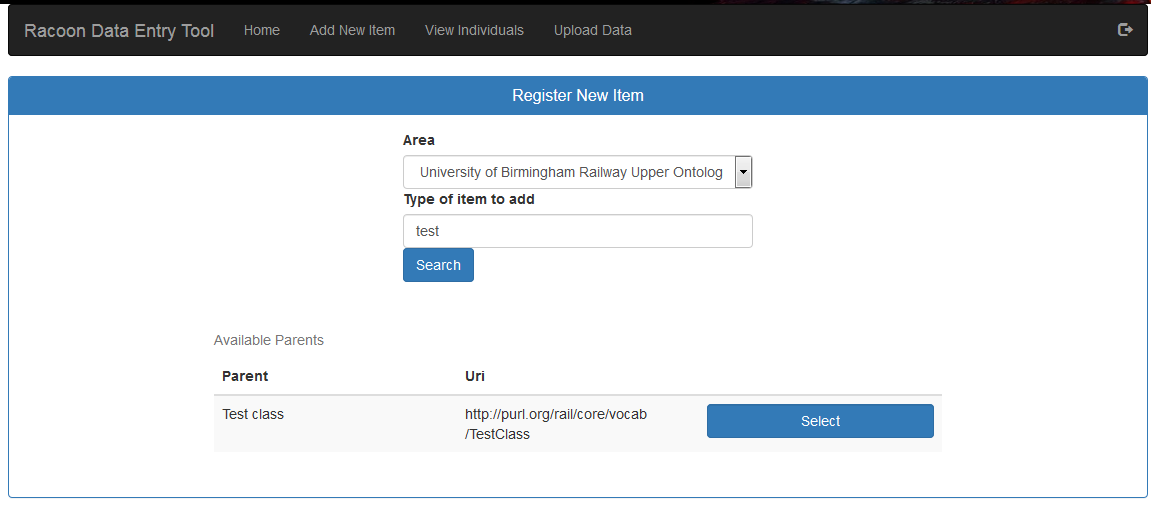
\includegraphics[max height=0.5\textheight,max width=\linewidth]{gfx/manToolAddingItem}} 
\caption[Manual Data Entry Tool Add item stage 1]{Manual Data Entry tool Adding an item stage one}
\label{fig:mtAddingItem}
\end{figure}

 \begin{figure}[!h]
\myfloatalign
{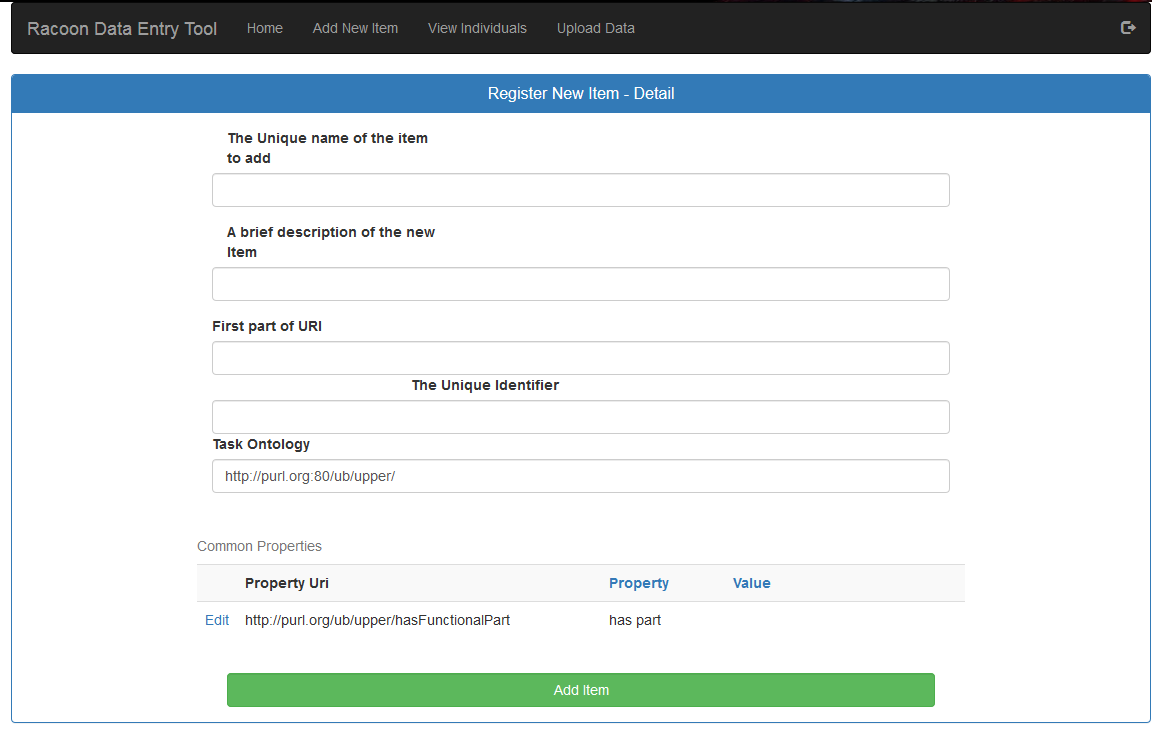
\includegraphics[max height=0.5\textheight,max width=\linewidth]{gfx/addItemDetail}} 
\caption[Manual Data Entry Tool Add item stage 2]{Manual Data Entry tool Adding an item stage two}
\label{fig:mtAddingItemDetail}
\end{figure}

